% The refined lattice spanned by i and 0.3 - 0.1i, obtained after
% replacing 1 by the smaller vector 0.3 - 0.1i: the mesh shrinks.
% The new basis vector is highlighted in red.
% Source: book/tex/alg-NT/classgrp.tex (§ Third proof) — asy figure.
\documentclass[border=2mm]{standalone}
\usepackage{tikz}
\begin{document}
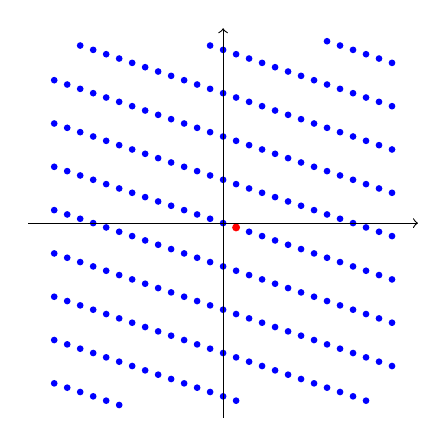
\begin{tikzpicture}[scale=0.55]
  \foreach \x in {-8,...,8}
    \foreach \y in {-20,...,20}
    {
      \pgfmathsetmacro{\px}{0.3*\y}
      \pgfmathsetmacro{\py}{\x-0.1*\y}
      \pgfmathparse{abs(\px)<=4.2 && abs(\py)<=4.2 ? 1 : 0}
      \ifnum\pgfmathresult=1
        \ifnum\x=0
          \ifnum\y=1
            \fill[red] (\px,\py) circle (2.6pt);
          \else
            \fill[blue] (\px,\py) circle (2.2pt);
          \fi
        \else
          \fill[blue] (\px,\py) circle (2.2pt);
        \fi
      \fi
    }
  \draw[->] (-4.5,0) -- (4.5,0);
  \draw[->] (0,-4.5) -- (0,4.5);
\end{tikzpicture}
\end{document}
